\documentclass[1p]{elsarticle_modified}
%\bibliographystyle{elsarticle-num}

%\usepackage[colorlinks]{hyperref}
%\usepackage{abbrmath_seonhwa} %\Abb, \Ascr, \Acal ,\Abf, \Afrak
\usepackage{amsfonts}
\usepackage{amssymb}
\usepackage{amsmath}
\usepackage{amsthm}
\usepackage{scalefnt}
\usepackage{amsbsy}
\usepackage{kotex}
\usepackage{caption}
\usepackage{subfig}
\usepackage{color}
\usepackage{graphicx}
\usepackage{xcolor} %% white, black, red, green, blue, cyan, magenta, yellow
\usepackage{float}
\usepackage{setspace}
\usepackage{hyperref}

\usepackage{tikz}
\usetikzlibrary{arrows}

\usepackage{multirow}
\usepackage{array} % fixed length table
\usepackage{hhline}

%%%%%%%%%%%%%%%%%%%%%
\makeatletter
\renewcommand*\env@matrix[1][\arraystretch]{%
	\edef\arraystretch{#1}%
	\hskip -\arraycolsep
	\let\@ifnextchar\new@ifnextchar
	\array{*\c@MaxMatrixCols c}}
\makeatother %https://tex.stackexchange.com/questions/14071/how-can-i-increase-the-line-spacing-in-a-matrix
%%%%%%%%%%%%%%%

\usepackage[normalem]{ulem}

\newcommand{\msout}[1]{\ifmmode\text{\sout{\ensuremath{#1}}}\else\sout{#1}\fi}
%SOURCE: \msout is \stkout macro in https://tex.stackexchange.com/questions/20609/strikeout-in-math-mode

\newcommand{\cancel}[1]{
	\ifmmode
	{\color{red}\msout{#1}}
	\else
	{\color{red}\sout{#1}}
	\fi
}

\newcommand{\add}[1]{
	{\color{blue}\uwave{#1}}
}

\newcommand{\replace}[2]{
	\ifmmode
	{\color{red}\msout{#1}}{\color{blue}\uwave{#2}}
	\else
	{\color{red}\sout{#1}}{\color{blue}\uwave{#2}}
	\fi
}

\newcommand{\Sol}{\mathcal{S}} %segment
\newcommand{\D}{D} %diagram
\newcommand{\A}{\mathcal{A}} %arc


%%%%%%%%%%%%%%%%%%%%%%%%%%%%%5 test

\def\sl{\operatorname{\textup{SL}}(2,\Cbb)}
\def\psl{\operatorname{\textup{PSL}}(2,\Cbb)}
\def\quan{\mkern 1mu \triangleright \mkern 1mu}

\theoremstyle{definition}
\newtheorem{thm}{Theorem}[section]
\newtheorem{prop}[thm]{Proposition}
\newtheorem{lem}[thm]{Lemma}
\newtheorem{ques}[thm]{Question}
\newtheorem{cor}[thm]{Corollary}
\newtheorem{defn}[thm]{Definition}
\newtheorem{exam}[thm]{Example}
\newtheorem{rmk}[thm]{Remark}
\newtheorem{alg}[thm]{Algorithm}

\newcommand{\I}{\sqrt{-1}}
\begin{document}

%\begin{frontmatter}
%
%\title{Boundary parabolic representations of knots up to 8 crossings}
%
%%% Group authors per affiliation:
%\author{Yunhi Cho} 
%\address{Department of Mathematics, University of Seoul, Seoul, Korea}
%\ead{yhcho@uos.ac.kr}
%
%
%\author{Seonhwa Kim} %\fnref{s_kim}}
%\address{Center for Geometry and Physics, Institute for Basic Science, Pohang, 37673, Korea}
%\ead{ryeona17@ibs.re.kr}
%
%\author{Hyuk Kim}
%\address{Department of Mathematical Sciences, Seoul National University, Seoul 08826, Korea}
%\ead{hyukkim@snu.ac.kr}
%
%\author{Seokbeom Yoon}
%\address{Department of Mathematical Sciences, Seoul National University, Seoul, 08826,  Korea}
%\ead{sbyoon15@snu.ac.kr}
%
%\begin{abstract}
%We find all boundary parabolic representation of knots up to 8 crossings.
%
%\end{abstract}
%\begin{keyword}
%    \MSC[2010] 57M25 
%\end{keyword}
%
%\end{frontmatter}

%\linenumbers
%\tableofcontents
%
\newcommand\colored[1]{\textcolor{white}{\rule[-0.35ex]{0.8em}{1.4ex}}\kern-0.8em\color{red} #1}%
%\newcommand\colored[1]{\textcolor{white}{ #1}\kern-2.17ex	\textcolor{white}{ #1}\kern-1.81ex	\textcolor{white}{ #1}\kern-2.15ex\color{red}#1	}

{\Large $\underline{12a_{0128}~(K12a_{0128})}$}

\setlength{\tabcolsep}{10pt}
\renewcommand{\arraystretch}{1.6}
\vspace{1cm}\begin{tabular}{m{100pt}>{\centering\arraybackslash}m{274pt}}
\multirow{5}{120pt}{
	\centering
	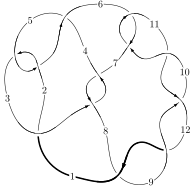
\includegraphics[width=112pt]{../../../GIT/diagram.site/Diagrams/png/929_12a_0128.png}\\
\ \ \ A knot diagram\footnotemark}&
\allowdisplaybreaks
\textbf{Linearized knot diagam} \\
\cline{2-2}
 &
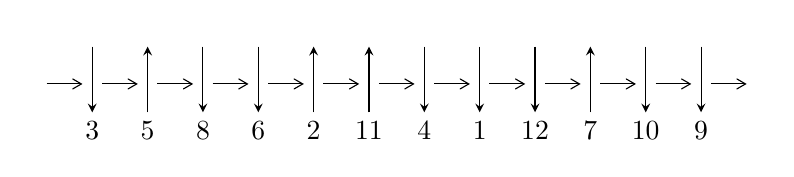
\begin{tikzpicture}[x=20pt, y=17pt]
	% nodes
	\node (C0) at (0, 0) {};
	\node (C1) at (1, 0) {};
	\node (C1U) at (1, +1) {};
	\node (C1D) at (1, -1) {3};

	\node (C2) at (2, 0) {};
	\node (C2U) at (2, +1) {};
	\node (C2D) at (2, -1) {5};

	\node (C3) at (3, 0) {};
	\node (C3U) at (3, +1) {};
	\node (C3D) at (3, -1) {8};

	\node (C4) at (4, 0) {};
	\node (C4U) at (4, +1) {};
	\node (C4D) at (4, -1) {6};

	\node (C5) at (5, 0) {};
	\node (C5U) at (5, +1) {};
	\node (C5D) at (5, -1) {2};

	\node (C6) at (6, 0) {};
	\node (C6U) at (6, +1) {};
	\node (C6D) at (6, -1) {11};

	\node (C7) at (7, 0) {};
	\node (C7U) at (7, +1) {};
	\node (C7D) at (7, -1) {4};

	\node (C8) at (8, 0) {};
	\node (C8U) at (8, +1) {};
	\node (C8D) at (8, -1) {1};

	\node (C9) at (9, 0) {};
	\node (C9U) at (9, +1) {};
	\node (C9D) at (9, -1) {12};

	\node (C10) at (10, 0) {};
	\node (C10U) at (10, +1) {};
	\node (C10D) at (10, -1) {7};

	\node (C11) at (11, 0) {};
	\node (C11U) at (11, +1) {};
	\node (C11D) at (11, -1) {10};

	\node (C12) at (12, 0) {};
	\node (C12U) at (12, +1) {};
	\node (C12D) at (12, -1) {9};
	\node (C13) at (13, 0) {};

	% arrows
	\draw[->,>={angle 60}]
	(C0) edge (C1) (C1) edge (C2) (C2) edge (C3) (C3) edge (C4) (C4) edge (C5) (C5) edge (C6) (C6) edge (C7) (C7) edge (C8) (C8) edge (C9) (C9) edge (C10) (C10) edge (C11) (C11) edge (C12) (C12) edge (C13) ;	\draw[->,>=stealth]
	(C1U) edge (C1D) (C2D) edge (C2U) (C3U) edge (C3D) (C4U) edge (C4D) (C5D) edge (C5U) (C6D) edge (C6U) (C7U) edge (C7D) (C8U) edge (C8D) (C9U) edge (C9D) (C10D) edge (C10U) (C11U) edge (C11D) (C12U) edge (C12D) ;
	\end{tikzpicture} \\
\hhline{~~} \\& 
\textbf{Solving Sequence} \\ \cline{2-2} 
 &
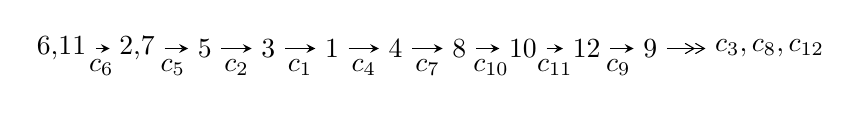
\begin{tikzpicture}[x=23pt, y=7pt]
	% node
	\node (A0) at (-1/8, 0) {6,11};
	\node (A1) at (17/16, 0) {2,7};
	\node (A2) at (17/8, 0) {5};
	\node (A3) at (25/8, 0) {3};
	\node (A4) at (33/8, 0) {1};
	\node (A5) at (41/8, 0) {4};
	\node (A6) at (49/8, 0) {8};
	\node (A7) at (57/8, 0) {10};
	\node (A8) at (65/8, 0) {12};
	\node (A9) at (73/8, 0) {9};
	\node (C1) at (1/2, -1) {$c_{6}$};
	\node (C2) at (13/8, -1) {$c_{5}$};
	\node (C3) at (21/8, -1) {$c_{2}$};
	\node (C4) at (29/8, -1) {$c_{1}$};
	\node (C5) at (37/8, -1) {$c_{4}$};
	\node (C6) at (45/8, -1) {$c_{7}$};
	\node (C7) at (53/8, -1) {$c_{10}$};
	\node (C8) at (61/8, -1) {$c_{11}$};
	\node (C9) at (69/8, -1) {$c_{9}$};
	\node (A10) at (11, 0) {$c_{3},c_{8},c_{12}$};

	% edge
	\draw[->,>=stealth]	
	(A0) edge (A1) (A1) edge (A2) (A2) edge (A3) (A3) edge (A4) (A4) edge (A5) (A5) edge (A6) (A6) edge (A7) (A7) edge (A8) (A8) edge (A9) ;
	\draw[->>,>={angle 60}]	
	(A9) edge (A10);
\end{tikzpicture} \\ 

\end{tabular} \\

\footnotetext{
The image of knot diagram is generated by the software ``\textbf{Draw programme}" developed by Andrew Bartholomew(\url{http://www.layer8.co.uk/maths/draw/index.htm\#Running-draw}), where we modified some parts for our purpose(\url{https://github.com/CATsTAILs/LinksPainter}).
}\phantom \\ \newline 
\centering \textbf{Ideals for irreducible components\footnotemark of $X_{\text{par}}$} 
 
\begin{align*}
I^u_{1}&=\langle 
- u^{56}+2 u^{55}+\cdots+2 b-4 u,\;u^{54}-2 u^{53}+\cdots+2 a-1,\;u^{58}-3 u^{57}+\cdots-3 u+1\rangle \\
I^u_{2}&=\langle 
u^2 a+u^2+b,\;- u^2 a- u^3+a^2+a u+u^2+a- u,\;u^4- u^3+u^2+1\rangle \\
\\
\end{align*}
\raggedright * 2 irreducible components of $\dim_{\mathbb{C}}=0$, with total 66 representations.\\
\footnotetext{All coefficients of polynomials are rational numbers. But the coefficients are sometimes approximated in decimal forms when there is not enough margin.}
\newpage
\renewcommand{\arraystretch}{1}
\centering \section*{I. $I^u_{1}= \langle - u^{56}+2 u^{55}+\cdots+2 b-4 u,\;u^{54}-2 u^{53}+\cdots+2 a-1,\;u^{58}-3 u^{57}+\cdots-3 u+1 \rangle$}
\flushleft \textbf{(i) Arc colorings}\\
\begin{tabular}{m{7pt} m{180pt} m{7pt} m{180pt} }
\flushright $a_{6}=$&$\begin{pmatrix}1\\0\end{pmatrix}$ \\
\flushright $a_{11}=$&$\begin{pmatrix}0\\u\end{pmatrix}$ \\
\flushright $a_{2}=$&$\begin{pmatrix}-\frac{1}{2} u^{54}+u^{53}+\cdots-\frac{1}{2} u+\frac{1}{2}\\\frac{1}{2} u^{56}- u^{55}+\cdots-\frac{5}{2} u^2+2 u\end{pmatrix}$ \\
\flushright $a_{7}=$&$\begin{pmatrix}1\\- u^2\end{pmatrix}$ \\
\flushright $a_{5}=$&$\begin{pmatrix}- u^{57}+\frac{3}{2} u^{56}+\cdots+\frac{13}{2} u-\frac{1}{2}\\- u^{57}+\frac{5}{2} u^{56}+\cdots+\frac{17}{2} u^2- u\end{pmatrix}$ \\
\flushright $a_{3}=$&$\begin{pmatrix}2 u^{56}-2 u^{55}+\cdots+\frac{15}{2} u-\frac{1}{2}\\-2 u^{57}+\frac{7}{2} u^{56}+\cdots+\frac{17}{2} u^2- u\end{pmatrix}$ \\
\flushright $a_{1}=$&$\begin{pmatrix}- u^7-2 u^3\\u^9+u^7+3 u^5+2 u^3+u\end{pmatrix}$ \\
\flushright $a_{4}=$&$\begin{pmatrix}-2 u^{57}+4 u^{56}+\cdots+\frac{11}{2} u-\frac{1}{2}\\- u^{57}+\frac{5}{2} u^{56}+\cdots+\frac{17}{2} u^2- u\end{pmatrix}$ \\
\flushright $a_{8}=$&$\begin{pmatrix}u^9+3 u^5+u\\- u^{11}- u^9-4 u^7-3 u^5-3 u^3- u\end{pmatrix}$ \\
\flushright $a_{10}=$&$\begin{pmatrix}- u\\u^3+u\end{pmatrix}$ \\
\flushright $a_{12}=$&$\begin{pmatrix}- u^3\\u^5+u^3+u\end{pmatrix}$ \\
\flushright $a_{9}=$&$\begin{pmatrix}- u^5- u\\u^7+u^5+2 u^3+u\end{pmatrix}$\\&\end{tabular}
\flushleft \textbf{(ii) Obstruction class $= -1$}\\~\\
\flushleft \textbf{(iii) Cusp Shapes $= -\frac{15}{2} u^{57}+12 u^{56}+\cdots-\frac{51}{2} u-\frac{1}{2}$}\\~\\
\newpage\renewcommand{\arraystretch}{1}
\flushleft \textbf{(iv) u-Polynomials at the component}\newline \\
\begin{tabular}{m{50pt}|m{274pt}}
Crossings & \hspace{64pt}u-Polynomials at each crossing \\
\hline $$\begin{aligned}c_{1},c_{4}\end{aligned}$$&$\begin{aligned}
&u^{58}+17 u^{57}+\cdots+49 u+1
\end{aligned}$\\
\hline $$\begin{aligned}c_{2},c_{5}\end{aligned}$$&$\begin{aligned}
&u^{58}+5 u^{57}+\cdots+u+1
\end{aligned}$\\
\hline $$\begin{aligned}c_{3},c_{7}\end{aligned}$$&$\begin{aligned}
&u^{58}- u^{57}+\cdots+384 u+256
\end{aligned}$\\
\hline $$\begin{aligned}c_{6},c_{10}\end{aligned}$$&$\begin{aligned}
&u^{58}-3 u^{57}+\cdots-3 u+1
\end{aligned}$\\
\hline $$\begin{aligned}c_{8},c_{9},c_{11}\\c_{12}\end{aligned}$$&$\begin{aligned}
&u^{58}+11 u^{57}+\cdots+21 u+1
\end{aligned}$\\
\hline
\end{tabular}\\~\\
\newpage\renewcommand{\arraystretch}{1}
\flushleft \textbf{(v) Riley Polynomials at the component}\newline \\
\begin{tabular}{m{50pt}|m{274pt}}
Crossings & \hspace{64pt}Riley Polynomials at each crossing \\
\hline $$\begin{aligned}c_{1},c_{4}\end{aligned}$$&$\begin{aligned}
&y^{58}+53 y^{57}+\cdots-451 y+1
\end{aligned}$\\
\hline $$\begin{aligned}c_{2},c_{5}\end{aligned}$$&$\begin{aligned}
&y^{58}+17 y^{57}+\cdots+49 y+1
\end{aligned}$\\
\hline $$\begin{aligned}c_{3},c_{7}\end{aligned}$$&$\begin{aligned}
&y^{58}+45 y^{57}+\cdots+475136 y+65536
\end{aligned}$\\
\hline $$\begin{aligned}c_{6},c_{10}\end{aligned}$$&$\begin{aligned}
&y^{58}+11 y^{57}+\cdots+21 y+1
\end{aligned}$\\
\hline $$\begin{aligned}c_{8},c_{9},c_{11}\\c_{12}\end{aligned}$$&$\begin{aligned}
&y^{58}+75 y^{57}+\cdots+45 y+1
\end{aligned}$\\
\hline
\end{tabular}\\~\\
\newpage\flushleft \textbf{(vi) Complex Volumes and Cusp Shapes}
$$\begin{array}{c|c|c}  
\text{Solutions to }I^u_{1}& \I (\text{vol} + \sqrt{-1}CS) & \text{Cusp shape}\\
 \hline 
\begin{aligned}
u &= \phantom{-}0.236171 + 0.966829 I \\
a &= -0.773305 + 0.432884 I \\
b &= -0.777739 + 0.842309 I\end{aligned}
 & \phantom{-}2.58788 - 0.06234 I & -2.29623 - 1.17460 I \\ \hline\begin{aligned}
u &= \phantom{-}0.236171 - 0.966829 I \\
a &= -0.773305 - 0.432884 I \\
b &= -0.777739 - 0.842309 I\end{aligned}
 & \phantom{-}2.58788 + 0.06234 I & -2.29623 + 1.17460 I \\ \hline\begin{aligned}
u &= -0.789321 + 0.603582 I \\
a &= \phantom{-}1.49361 - 0.38105 I \\
b &= -0.866625 + 0.810195 I\end{aligned}
 & \phantom{-}8.82733 - 0.53338 I & \phantom{-}4.24509 + 1.90410 I \\ \hline\begin{aligned}
u &= -0.789321 - 0.603582 I \\
a &= \phantom{-}1.49361 + 0.38105 I \\
b &= -0.866625 - 0.810195 I\end{aligned}
 & \phantom{-}8.82733 + 0.53338 I & \phantom{-}4.24509 - 1.90410 I \\ \hline\begin{aligned}
u &= -0.557363 + 0.839839 I \\
a &= -1.49324 - 1.38719 I \\
b &= \phantom{-}0.257230 - 1.060260 I\end{aligned}
 & \phantom{-}0.27509 - 5.53347 I & -2.68605 + 8.82067 I \\ \hline\begin{aligned}
u &= -0.557363 - 0.839839 I \\
a &= -1.49324 + 1.38719 I \\
b &= \phantom{-}0.257230 + 1.060260 I\end{aligned}
 & \phantom{-}0.27509 + 5.53347 I & -2.68605 - 8.82067 I \\ \hline\begin{aligned}
u &= \phantom{-}0.191407 + 0.973334 I \\
a &= \phantom{-}0.61484 - 1.91027 I \\
b &= -0.761623 - 0.924314 I\end{aligned}
 & \phantom{-}2.33477 + 5.75175 I & -3.31343 - 6.58381 I \\ \hline\begin{aligned}
u &= \phantom{-}0.191407 - 0.973334 I \\
a &= \phantom{-}0.61484 + 1.91027 I \\
b &= -0.761623 + 0.924314 I\end{aligned}
 & \phantom{-}2.33477 - 5.75175 I & -3.31343 + 6.58381 I \\ \hline\begin{aligned}
u &= -0.650775 + 0.773636 I \\
a &= -0.562703 - 0.501035 I \\
b &= \phantom{-}0.694164 - 0.069962 I\end{aligned}
 & \phantom{-}3.85863 - 2.42965 I & \phantom{-}4.20800 + 3.88872 I \\ \hline\begin{aligned}
u &= -0.650775 - 0.773636 I \\
a &= -0.562703 + 0.501035 I \\
b &= \phantom{-}0.694164 + 0.069962 I\end{aligned}
 & \phantom{-}3.85863 + 2.42965 I & \phantom{-}4.20800 - 3.88872 I\\
 \hline 
 \end{array}$$\newpage$$\begin{array}{c|c|c}  
\text{Solutions to }I^u_{1}& \I (\text{vol} + \sqrt{-1}CS) & \text{Cusp shape}\\
 \hline 
\begin{aligned}
u &= \phantom{-}0.621083 + 0.799921 I \\
a &= -2.68797 + 0.17282 I \\
b &= \phantom{-}0.714179 + 0.895252 I\end{aligned}
 & \phantom{-}3.02078 + 5.11389 I & \phantom{-0.000000 } 0. - 6.57141 I \\ \hline\begin{aligned}
u &= \phantom{-}0.621083 - 0.799921 I \\
a &= -2.68797 - 0.17282 I \\
b &= \phantom{-}0.714179 - 0.895252 I\end{aligned}
 & \phantom{-}3.02078 - 5.11389 I & \phantom{-0.000000 -}0. + 6.57141 I \\ \hline\begin{aligned}
u &= \phantom{-}0.641113 + 0.736885 I \\
a &= -1.05326 + 1.50993 I \\
b &= \phantom{-}0.727655 - 0.829091 I\end{aligned}
 & \phantom{-}3.22659 - 0.38005 I & \phantom{-}1.076438 - 0.381418 I \\ \hline\begin{aligned}
u &= \phantom{-}0.641113 - 0.736885 I \\
a &= -1.05326 - 1.50993 I \\
b &= \phantom{-}0.727655 + 0.829091 I\end{aligned}
 & \phantom{-}3.22659 + 0.38005 I & \phantom{-}1.076438 + 0.381418 I \\ \hline\begin{aligned}
u &= -0.784621 + 0.562056 I \\
a &= \phantom{-}1.34703 + 0.49250 I \\
b &= -0.805827 - 0.978477 I\end{aligned}
 & \phantom{-}8.30451 + 5.68111 I & \phantom{-}3.40199 - 3.19190 I \\ \hline\begin{aligned}
u &= -0.784621 - 0.562056 I \\
a &= \phantom{-}1.34703 - 0.49250 I \\
b &= -0.805827 + 0.978477 I\end{aligned}
 & \phantom{-}8.30451 - 5.68111 I & \phantom{-}3.40199 + 3.19190 I \\ \hline\begin{aligned}
u &= \phantom{-}0.419617 + 0.831418 I \\
a &= \phantom{-}1.92901 - 0.95806 I \\
b &= -0.048744 - 0.737006 I\end{aligned}
 & -1.20572 + 2.00199 I & -7.02325 - 3.53170 I \\ \hline\begin{aligned}
u &= \phantom{-}0.419617 - 0.831418 I \\
a &= \phantom{-}1.92901 + 0.95806 I \\
b &= -0.048744 + 0.737006 I\end{aligned}
 & -1.20572 - 2.00199 I & -7.02325 + 3.53170 I \\ \hline\begin{aligned}
u &= -0.584881 + 0.658903 I \\
a &= \phantom{-}0.148792 + 0.449303 I \\
b &= \phantom{-}0.354250 + 1.034950 I\end{aligned}
 & \phantom{-}0.86366 + 1.17340 I & \phantom{-}0.879783 - 1.104139 I \\ \hline\begin{aligned}
u &= -0.584881 - 0.658903 I \\
a &= \phantom{-}0.148792 - 0.449303 I \\
b &= \phantom{-}0.354250 - 1.034950 I\end{aligned}
 & \phantom{-}0.86366 - 1.17340 I & \phantom{-}0.879783 + 1.104139 I\\
 \hline 
 \end{array}$$\newpage$$\begin{array}{c|c|c}  
\text{Solutions to }I^u_{1}& \I (\text{vol} + \sqrt{-1}CS) & \text{Cusp shape}\\
 \hline 
\begin{aligned}
u &= -0.598169 + 0.963503 I \\
a &= \phantom{-}2.16232 + 1.27766 I \\
b &= -0.779295 + 0.996450 I\end{aligned}
 & \phantom{-}6.97066 - 10.76520 I & \phantom{-0.000000 } 0 \\ \hline\begin{aligned}
u &= -0.598169 - 0.963503 I \\
a &= \phantom{-}2.16232 - 1.27766 I \\
b &= -0.779295 - 0.996450 I\end{aligned}
 & \phantom{-}6.97066 + 10.76520 I & \phantom{-0.000000 } 0 \\ \hline\begin{aligned}
u &= -0.627970 + 0.950567 I \\
a &= -0.095056 + 1.088790 I \\
b &= -0.853835 - 0.767019 I\end{aligned}
 & \phantom{-}7.67631 - 4.67661 I & \phantom{-0.000000 } 0 \\ \hline\begin{aligned}
u &= -0.627970 - 0.950567 I \\
a &= -0.095056 - 1.088790 I \\
b &= -0.853835 + 0.767019 I\end{aligned}
 & \phantom{-}7.67631 + 4.67661 I & \phantom{-0.000000 } 0 \\ \hline\begin{aligned}
u &= \phantom{-}0.071034 + 0.820875 I \\
a &= \phantom{-}0.48145 + 2.63173 I \\
b &= \phantom{-}0.134528 + 0.904687 I\end{aligned}
 & -2.92758 + 1.95595 I & -11.89625 - 4.81261 I \\ \hline\begin{aligned}
u &= \phantom{-}0.071034 - 0.820875 I \\
a &= \phantom{-}0.48145 - 2.63173 I \\
b &= \phantom{-}0.134528 - 0.904687 I\end{aligned}
 & -2.92758 - 1.95595 I & -11.89625 + 4.81261 I \\ \hline\begin{aligned}
u &= -0.864927 + 0.895250 I \\
a &= \phantom{-}0.697824 + 0.131404 I \\
b &= -0.302360 - 0.659717 I\end{aligned}
 & \phantom{-}6.57199 - 1.97448 I & \phantom{-0.000000 } 0 \\ \hline\begin{aligned}
u &= -0.864927 - 0.895250 I \\
a &= \phantom{-}0.697824 - 0.131404 I \\
b &= -0.302360 + 0.659717 I\end{aligned}
 & \phantom{-}6.57199 + 1.97448 I & \phantom{-0.000000 } 0 \\ \hline\begin{aligned}
u &= -0.851879 + 0.930952 I \\
a &= \phantom{-}1.53417 + 0.29283 I \\
b &= -0.284323 + 0.694959 I\end{aligned}
 & \phantom{-}6.46068 - 4.39375 I & \phantom{-0.000000 } 0 \\ \hline\begin{aligned}
u &= -0.851879 - 0.930952 I \\
a &= \phantom{-}1.53417 - 0.29283 I \\
b &= -0.284323 - 0.694959 I\end{aligned}
 & \phantom{-}6.46068 + 4.39375 I & \phantom{-0.000000 } 0\\
 \hline 
 \end{array}$$\newpage$$\begin{array}{c|c|c}  
\text{Solutions to }I^u_{1}& \I (\text{vol} + \sqrt{-1}CS) & \text{Cusp shape}\\
 \hline 
\begin{aligned}
u &= \phantom{-}0.910198 + 0.920175 I \\
a &= -0.1069100 - 0.0175219 I \\
b &= \phantom{-}0.318618 - 1.173080 I\end{aligned}
 & \phantom{-}9.62869 - 0.79499 I & \phantom{-0.000000 } 0 \\ \hline\begin{aligned}
u &= \phantom{-}0.910198 - 0.920175 I \\
a &= -0.1069100 + 0.0175219 I \\
b &= \phantom{-}0.318618 + 1.173080 I\end{aligned}
 & \phantom{-}9.62869 + 0.79499 I & \phantom{-0.000000 } 0 \\ \hline\begin{aligned}
u &= \phantom{-}0.325035 + 0.621241 I \\
a &= \phantom{-}0.691818 + 0.030726 I \\
b &= -0.045053 + 0.234286 I\end{aligned}
 & -0.201748 + 1.112070 I & -3.30409 - 5.91204 I \\ \hline\begin{aligned}
u &= \phantom{-}0.325035 - 0.621241 I \\
a &= \phantom{-}0.691818 - 0.030726 I \\
b &= -0.045053 - 0.234286 I\end{aligned}
 & -0.201748 - 1.112070 I & -3.30409 + 5.91204 I \\ \hline\begin{aligned}
u &= \phantom{-}0.942009 + 0.898668 I \\
a &= \phantom{-}1.31780 - 0.56148 I \\
b &= -0.811125 + 1.045670 I\end{aligned}
 & \phantom{-}17.4170 - 7.1616 I & \phantom{-0.000000 } 0 \\ \hline\begin{aligned}
u &= \phantom{-}0.942009 - 0.898668 I \\
a &= \phantom{-}1.31780 + 0.56148 I \\
b &= -0.811125 - 1.045670 I\end{aligned}
 & \phantom{-}17.4170 + 7.1616 I & \phantom{-0.000000 } 0 \\ \hline\begin{aligned}
u &= \phantom{-}0.895499 + 0.949477 I \\
a &= -1.43215 + 0.42653 I \\
b &= \phantom{-}0.303547 + 1.175220 I\end{aligned}
 & \phantom{-}9.53363 + 7.45134 I & \phantom{-0.000000 } 0 \\ \hline\begin{aligned}
u &= \phantom{-}0.895499 - 0.949477 I \\
a &= -1.43215 - 0.42653 I \\
b &= \phantom{-}0.303547 - 1.175220 I\end{aligned}
 & \phantom{-}9.53363 - 7.45134 I & \phantom{-0.000000 } 0 \\ \hline\begin{aligned}
u &= -0.914772 + 0.933791 I \\
a &= -1.32356 - 1.26003 I \\
b &= \phantom{-}0.823322 + 0.892050 I\end{aligned}
 & \phantom{-}12.70460 - 0.29180 I & \phantom{-0.000000 } 0 \\ \hline\begin{aligned}
u &= -0.914772 - 0.933791 I \\
a &= -1.32356 + 1.26003 I \\
b &= \phantom{-}0.823322 - 0.892050 I\end{aligned}
 & \phantom{-}12.70460 + 0.29180 I & \phantom{-0.000000 } 0\\
 \hline 
 \end{array}$$\newpage$$\begin{array}{c|c|c}  
\text{Solutions to }I^u_{1}& \I (\text{vol} + \sqrt{-1}CS) & \text{Cusp shape}\\
 \hline 
\begin{aligned}
u &= \phantom{-}0.690394 + 0.030120 I \\
a &= \phantom{-}1.39889 + 0.41674 I \\
b &= -0.809868 - 0.894099 I\end{aligned}
 & \phantom{-}5.73169 + 3.03027 I & \phantom{-}4.19424 - 2.78424 I \\ \hline\begin{aligned}
u &= \phantom{-}0.690394 - 0.030120 I \\
a &= \phantom{-}1.39889 - 0.41674 I \\
b &= -0.809868 + 0.894099 I\end{aligned}
 & \phantom{-}5.73169 - 3.03027 I & \phantom{-}4.19424 + 2.78424 I \\ \hline\begin{aligned}
u &= \phantom{-}0.942436 + 0.909290 I \\
a &= \phantom{-}1.57800 + 0.37798 I \\
b &= -0.942649 - 0.753265 I\end{aligned}
 & \phantom{-}18.3412 - 0.7119 I & \phantom{-0.000000 } 0 \\ \hline\begin{aligned}
u &= \phantom{-}0.942436 - 0.909290 I \\
a &= \phantom{-}1.57800 - 0.37798 I \\
b &= -0.942649 + 0.753265 I\end{aligned}
 & \phantom{-}18.3412 + 0.7119 I & \phantom{-0.000000 } 0 \\ \hline\begin{aligned}
u &= -0.908706 + 0.945270 I \\
a &= -2.36231 + 0.27916 I \\
b &= \phantom{-}0.818870 - 0.903943 I\end{aligned}
 & \phantom{-}12.6670 - 6.4226 I & \phantom{-0.000000 } 0 \\ \hline\begin{aligned}
u &= -0.908706 - 0.945270 I \\
a &= -2.36231 - 0.27916 I \\
b &= \phantom{-}0.818870 + 0.903943 I\end{aligned}
 & \phantom{-}12.6670 + 6.4226 I & \phantom{-0.000000 } 0 \\ \hline\begin{aligned}
u &= \phantom{-}0.914486 + 0.940989 I \\
a &= -1.045780 + 0.497688 I \\
b &= \phantom{-}0.892652 + 0.010539 I\end{aligned}
 & \phantom{-}13.59950 + 3.36619 I & \phantom{-0.000000 } 0 \\ \hline\begin{aligned}
u &= \phantom{-}0.914486 - 0.940989 I \\
a &= -1.045780 - 0.497688 I \\
b &= \phantom{-}0.892652 - 0.010539 I\end{aligned}
 & \phantom{-}13.59950 - 3.36619 I & \phantom{-0.000000 } 0 \\ \hline\begin{aligned}
u &= \phantom{-}0.895550 + 0.983231 I \\
a &= \phantom{-}2.40578 - 0.45339 I \\
b &= -0.803885 - 1.049880 I\end{aligned}
 & \phantom{-}17.1389 + 13.9172 I & \phantom{-0.000000 } 0 \\ \hline\begin{aligned}
u &= \phantom{-}0.895550 - 0.983231 I \\
a &= \phantom{-}2.40578 + 0.45339 I \\
b &= -0.803885 + 1.049880 I\end{aligned}
 & \phantom{-}17.1389 - 13.9172 I & \phantom{-0.000000 } 0\\
 \hline 
 \end{array}$$\newpage$$\begin{array}{c|c|c}  
\text{Solutions to }I^u_{1}& \I (\text{vol} + \sqrt{-1}CS) & \text{Cusp shape}\\
 \hline 
\begin{aligned}
u &= \phantom{-}0.903709 + 0.978699 I \\
a &= \phantom{-}0.66497 - 1.36041 I \\
b &= -0.941425 + 0.741601 I\end{aligned}
 & \phantom{-}18.1123 + 7.4971 I & \phantom{-0.000000 } 0 \\ \hline\begin{aligned}
u &= \phantom{-}0.903709 - 0.978699 I \\
a &= \phantom{-}0.66497 + 1.36041 I \\
b &= -0.941425 - 0.741601 I\end{aligned}
 & \phantom{-}18.1123 - 7.4971 I & \phantom{-0.000000 } 0 \\ \hline\begin{aligned}
u &= -0.138946 + 0.644931 I \\
a &= -2.02349 - 2.26505 I \\
b &= \phantom{-}0.559591 - 0.926866 I\end{aligned}
 & -0.64003 - 2.84760 I & -8.08127 + 0.14345 I \\ \hline\begin{aligned}
u &= -0.138946 - 0.644931 I \\
a &= -2.02349 + 2.26505 I \\
b &= \phantom{-}0.559591 + 0.926866 I\end{aligned}
 & -0.64003 + 2.84760 I & -8.08127 - 0.14345 I \\ \hline\begin{aligned}
u &= \phantom{-}0.344616 + 0.363333 I \\
a &= \phantom{-}0.547401 - 0.207447 I \\
b &= \phantom{-}0.251942 + 0.577672 I\end{aligned}
 & -0.068529 + 1.208380 I & -0.22566 - 4.75539 I \\ \hline\begin{aligned}
u &= \phantom{-}0.344616 - 0.363333 I \\
a &= \phantom{-}0.547401 + 0.207447 I \\
b &= \phantom{-}0.251942 - 0.577672 I\end{aligned}
 & -0.068529 - 1.208380 I & -0.22566 + 4.75539 I \\ \hline\begin{aligned}
u &= -0.172028 + 0.378457 I \\
a &= \phantom{-}0.94604 - 1.19928 I \\
b &= \phantom{-}0.483828 + 0.745563 I\end{aligned}
 & \phantom{-}0.00258 + 1.44884 I & -2.25105 - 5.51745 I \\ \hline\begin{aligned}
u &= -0.172028 - 0.378457 I \\
a &= \phantom{-}0.94604 + 1.19928 I \\
b &= \phantom{-}0.483828 - 0.745563 I\end{aligned}
 & \phantom{-}0.00258 - 1.44884 I & -2.25105 + 5.51745 I\\
 \hline 
 \end{array}$$\newpage\newpage\renewcommand{\arraystretch}{1}
\centering \section*{II. $I^u_{2}= \langle u^2 a+u^2+b,\;- u^2 a- u^3+a^2+a u+u^2+a- u,\;u^4- u^3+u^2+1 \rangle$}
\flushleft \textbf{(i) Arc colorings}\\
\begin{tabular}{m{7pt} m{180pt} m{7pt} m{180pt} }
\flushright $a_{6}=$&$\begin{pmatrix}1\\0\end{pmatrix}$ \\
\flushright $a_{11}=$&$\begin{pmatrix}0\\u\end{pmatrix}$ \\
\flushright $a_{2}=$&$\begin{pmatrix}a\\- u^2 a- u^2\end{pmatrix}$ \\
\flushright $a_{7}=$&$\begin{pmatrix}1\\- u^2\end{pmatrix}$ \\
\flushright $a_{5}=$&$\begin{pmatrix}u^2 a+a+u+1\\- u^2 a- u^2-1\end{pmatrix}$ \\
\flushright $a_{3}=$&$\begin{pmatrix}- u^2+a+u\\- u^2 a- u^2-1\end{pmatrix}$ \\
\flushright $a_{1}=$&$\begin{pmatrix}-1\\0\end{pmatrix}$ \\
\flushright $a_{4}=$&$\begin{pmatrix}- u^2+a+u\\- u^2 a- u^2-1\end{pmatrix}$ \\
\flushright $a_{8}=$&$\begin{pmatrix}1\\- u^2\end{pmatrix}$ \\
\flushright $a_{10}=$&$\begin{pmatrix}- u\\u^3+u\end{pmatrix}$ \\
\flushright $a_{12}=$&$\begin{pmatrix}- u^3\\u^3- u^2-1\end{pmatrix}$ \\
\flushright $a_{9}=$&$\begin{pmatrix}u^2+1\\- u^2\end{pmatrix}$\\&\end{tabular}
\flushleft \textbf{(ii) Obstruction class $= 1$}\\~\\
\flushleft \textbf{(iii) Cusp Shapes $= u^3 a+4 u^2 a+2 a u+u^2- a+6 u-2$}\\~\\
\newpage\renewcommand{\arraystretch}{1}
\flushleft \textbf{(iv) u-Polynomials at the component}\newline \\
\begin{tabular}{m{50pt}|m{274pt}}
Crossings & \hspace{64pt}u-Polynomials at each crossing \\
\hline $$\begin{aligned}c_{1},c_{4},c_{5}\end{aligned}$$&$\begin{aligned}
&(u^2- u+1)^4
\end{aligned}$\\
\hline $$\begin{aligned}c_{2}\end{aligned}$$&$\begin{aligned}
&(u^2+u+1)^4
\end{aligned}$\\
\hline $$\begin{aligned}c_{3},c_{7}\end{aligned}$$&$\begin{aligned}
&u^8
\end{aligned}$\\
\hline $$\begin{aligned}c_{6}\end{aligned}$$&$\begin{aligned}
&(u^4- u^3+u^2+1)^2
\end{aligned}$\\
\hline $$\begin{aligned}c_{8},c_{9}\end{aligned}$$&$\begin{aligned}
&(u^4- u^3+3 u^2-2 u+1)^2
\end{aligned}$\\
\hline $$\begin{aligned}c_{10}\end{aligned}$$&$\begin{aligned}
&(u^4+u^3+u^2+1)^2
\end{aligned}$\\
\hline $$\begin{aligned}c_{11},c_{12}\end{aligned}$$&$\begin{aligned}
&(u^4+u^3+3 u^2+2 u+1)^2
\end{aligned}$\\
\hline
\end{tabular}\\~\\
\newpage\renewcommand{\arraystretch}{1}
\flushleft \textbf{(v) Riley Polynomials at the component}\newline \\
\begin{tabular}{m{50pt}|m{274pt}}
Crossings & \hspace{64pt}Riley Polynomials at each crossing \\
\hline $$\begin{aligned}c_{1},c_{2},c_{4}\\c_{5}\end{aligned}$$&$\begin{aligned}
&(y^2+y+1)^4
\end{aligned}$\\
\hline $$\begin{aligned}c_{3},c_{7}\end{aligned}$$&$\begin{aligned}
&y^8
\end{aligned}$\\
\hline $$\begin{aligned}c_{6},c_{10}\end{aligned}$$&$\begin{aligned}
&(y^4+y^3+3 y^2+2 y+1)^2
\end{aligned}$\\
\hline $$\begin{aligned}c_{8},c_{9},c_{11}\\c_{12}\end{aligned}$$&$\begin{aligned}
&(y^4+5 y^3+7 y^2+2 y+1)^2
\end{aligned}$\\
\hline
\end{tabular}\\~\\
\newpage\flushleft \textbf{(vi) Complex Volumes and Cusp Shapes}
$$\begin{array}{c|c|c}  
\text{Solutions to }I^u_{2}& \I (\text{vol} + \sqrt{-1}CS) & \text{Cusp shape}\\
 \hline 
\begin{aligned}
u &= -0.351808 + 0.720342 I \\
a &= \phantom{-}0.541116 + 0.214920 I \\
b &= \phantom{-}0.500000 + 0.866025 I\end{aligned}
 & -0.211005 + 0.614778 I & -5.86133 + 2.84273 I \\ \hline\begin{aligned}
u &= -0.351808 + 0.720342 I \\
a &= -1.58443 - 1.44211 I \\
b &= \phantom{-}0.500000 - 0.866025 I\end{aligned}
 & -0.21101 - 3.44499 I & -1.10064 + 8.92228 I \\ \hline\begin{aligned}
u &= -0.351808 - 0.720342 I \\
a &= \phantom{-}0.541116 - 0.214920 I \\
b &= \phantom{-}0.500000 - 0.866025 I\end{aligned}
 & -0.211005 - 0.614778 I & -5.86133 - 2.84273 I \\ \hline\begin{aligned}
u &= -0.351808 - 0.720342 I \\
a &= -1.58443 + 1.44211 I \\
b &= \phantom{-}0.500000 + 0.866025 I\end{aligned}
 & -0.21101 + 3.44499 I & -1.10064 - 8.92228 I \\ \hline\begin{aligned}
u &= \phantom{-}0.851808 + 0.911292 I \\
a &= -0.423047 + 0.283088 I \\
b &= \phantom{-}0.500000 - 0.866025 I\end{aligned}
 & \phantom{-}6.79074 + 1.13408 I & \phantom{-}0.90087 + 2.75771 I \\ \hline\begin{aligned}
u &= \phantom{-}0.851808 + 0.911292 I \\
a &= -1.53364 + 0.35811 I \\
b &= \phantom{-}0.500000 + 0.866025 I\end{aligned}
 & \phantom{-}6.79074 + 5.19385 I & \phantom{-}1.56110 - 7.61722 I \\ \hline\begin{aligned}
u &= \phantom{-}0.851808 - 0.911292 I \\
a &= -0.423047 - 0.283088 I \\
b &= \phantom{-}0.500000 + 0.866025 I\end{aligned}
 & \phantom{-}6.79074 - 1.13408 I & \phantom{-}0.90087 - 2.75771 I \\ \hline\begin{aligned}
u &= \phantom{-}0.851808 - 0.911292 I \\
a &= -1.53364 - 0.35811 I \\
b &= \phantom{-}0.500000 - 0.866025 I\end{aligned}
 & \phantom{-}6.79074 - 5.19385 I & \phantom{-}1.56110 + 7.61722 I\\
 \hline 
 \end{array}$$\newpage
\newpage\renewcommand{\arraystretch}{1}
\centering \section*{ III. u-Polynomials}
\begin{tabular}{m{50pt}|m{274pt}}
Crossings & \hspace{64pt}u-Polynomials at each crossing \\
\hline $$\begin{aligned}c_{1},c_{4}\end{aligned}$$&$\begin{aligned}
&((u^2- u+1)^4)(u^{58}+17 u^{57}+\cdots+49 u+1)
\end{aligned}$\\
\hline $$\begin{aligned}c_{2}\end{aligned}$$&$\begin{aligned}
&((u^2+u+1)^4)(u^{58}+5 u^{57}+\cdots+u+1)
\end{aligned}$\\
\hline $$\begin{aligned}c_{3},c_{7}\end{aligned}$$&$\begin{aligned}
&u^8(u^{58}- u^{57}+\cdots+384 u+256)
\end{aligned}$\\
\hline $$\begin{aligned}c_{5}\end{aligned}$$&$\begin{aligned}
&((u^2- u+1)^4)(u^{58}+5 u^{57}+\cdots+u+1)
\end{aligned}$\\
\hline $$\begin{aligned}c_{6}\end{aligned}$$&$\begin{aligned}
&((u^4- u^3+u^2+1)^2)(u^{58}-3 u^{57}+\cdots-3 u+1)
\end{aligned}$\\
\hline $$\begin{aligned}c_{8},c_{9}\end{aligned}$$&$\begin{aligned}
&((u^4- u^3+3 u^2-2 u+1)^2)(u^{58}+11 u^{57}+\cdots+21 u+1)
\end{aligned}$\\
\hline $$\begin{aligned}c_{10}\end{aligned}$$&$\begin{aligned}
&((u^4+u^3+u^2+1)^2)(u^{58}-3 u^{57}+\cdots-3 u+1)
\end{aligned}$\\
\hline $$\begin{aligned}c_{11},c_{12}\end{aligned}$$&$\begin{aligned}
&((u^4+u^3+3 u^2+2 u+1)^2)(u^{58}+11 u^{57}+\cdots+21 u+1)
\end{aligned}$\\
\hline
\end{tabular}\newpage\renewcommand{\arraystretch}{1}
\centering \section*{ IV. Riley Polynomials}
\begin{tabular}{m{50pt}|m{274pt}}
Crossings & \hspace{64pt}Riley Polynomials at each crossing \\
\hline $$\begin{aligned}c_{1},c_{4}\end{aligned}$$&$\begin{aligned}
&((y^2+y+1)^4)(y^{58}+53 y^{57}+\cdots-451 y+1)
\end{aligned}$\\
\hline $$\begin{aligned}c_{2},c_{5}\end{aligned}$$&$\begin{aligned}
&((y^2+y+1)^4)(y^{58}+17 y^{57}+\cdots+49 y+1)
\end{aligned}$\\
\hline $$\begin{aligned}c_{3},c_{7}\end{aligned}$$&$\begin{aligned}
&y^8(y^{58}+45 y^{57}+\cdots+475136 y+65536)
\end{aligned}$\\
\hline $$\begin{aligned}c_{6},c_{10}\end{aligned}$$&$\begin{aligned}
&((y^4+y^3+3 y^2+2 y+1)^2)(y^{58}+11 y^{57}+\cdots+21 y+1)
\end{aligned}$\\
\hline $$\begin{aligned}c_{8},c_{9},c_{11}\\c_{12}\end{aligned}$$&$\begin{aligned}
&((y^4+5 y^3+7 y^2+2 y+1)^2)(y^{58}+75 y^{57}+\cdots+45 y+1)
\end{aligned}$\\
\hline
\end{tabular}
\vskip 2pc
\end{document}